\begin{frame}[allowframebreaks]{Unsupervised Learning - Applications}
    Unsupervised learning is used in various fields and applications, including:
    \begin{itemize}
        \item \textbf{Visualisation}: Identifying and making accessiblge useful hidden structures in the data.
        \item \textbf{Anomaly Detection}: Identifying factory components that are likely to break soon.
        \item \textbf{Signal denoising}: Extracting human speech from a noisy recording.
        \item \textbf{Generative Models}: Learning to generate new data points similar to the training data.
        \item \textbf{Feature Learning}: Automatically discovering useful representations of the data.
        \item \textbf{Data Preprocessing}: Cleaning and transforming data for better performance in supervised learning tasks.
    \end{itemize}
\end{frame}

\begin{frame}{Application: Discovering Structure in Digits}
    \begin{figure}
    \centering
    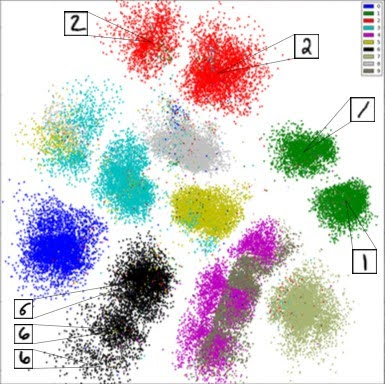
\includegraphics[width=0.8\textwidth,height=0.75\textheight,keepaspectratio]{images/dul-app-discover-structure.jpg}
    \caption{Unsupervised learning can discover structure in digits without any labels.}
    \end{figure}
\end{frame}

\begin{frame}{Application: DNA Analysis}
    \begin{figure}
    \centering
    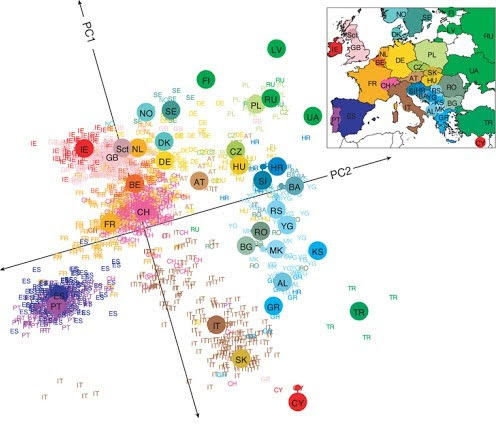
\includegraphics[width=0.8\textwidth,height=0.75\textheight,keepaspectratio]{images/dul-app-dim-reduce.jpg}
    \caption{Dimensionality reduction applied to DNA reveal the geography of European countries.}
    \end{figure}
\end{frame}